\documentclass{article}
\usepackage{graphicx}
\usepackage[font=small, labelfont=bf]{caption}
\usepackage{subcaption}
\usepackage{amsmath, amssymb, amsthm}
\usepackage{array}
\usepackage{tabularx}
\usepackage{longtable}
\usepackage{booktabs}
\usepackage{listings}
\usepackage[section]{placeins}
\usepackage[colorinlistoftodos]{todonotes}

\newcolumntype{L}{>{\raggedright\arraybackslash}X}

\lstset{
    basicstyle=\ttfamily\scriptsize,
    keepspaces=true,
    columns=fullflexible,
    breaklines=true,
    breakatwhitespace=false,
    frame=single,
    framesep=5pt,
    xleftmargin=6pt,
    xrightmargin=6pt,
    aboveskip=10pt,
    belowskip=10pt,
    captionpos=b
}

\title{CGR Report 3}
\author{Evan Brown}
\date{November 2026}

\begin{document}

\maketitle

\section*{Prompt Development}
Generative AI was used in architecting, implementing and explaining the code. Claude Code's Opus 5.5 was prompted with the CWSpec2026.pdf file and was tasked with implementing the features of module 3, which it did without intervention except for the installation of PBRT-v4 which was needed for comparison in the test suite.

\section{Acceleration Data Structure -- Bounding Volume Hierarchy}

\subsection{Key Design Decision}

\subsubsection{Class Structure}
Our implementation of the bounding volume hierarchy was through class \verb|BVH|, which lived inside the \verb|source/scene.cpp| and \verb|source/scene.h| files. It is implemented with attributes \verb|nodes_| to store the nodes, and \verb|prims_| to sequentially store the primitives at each leaf node. It also has methods \verb|BVH::build| to construct the tree, \verb|BVH::intersect| to test for the closest hit and \verb|BVH::occulded| to test for any hit.

\subsubsection{Algorithm Choices}
The most interesting part is the construction of the accelerating data structure. \verb|BVH::build| first computes the bounding box and centroid for every primitive and caches it. It then recursively calls \verb|BVH::buildRec| on an array of primitives creates a \verb|Node| which encloses them all, always picks the longest axis of the box around their centroids and sorts the centroid of each into 16 bins, and computes based the surface area heuristic where between these 16 bins it will subdivide into two new vectors of primitives. It will then recursively call \verb|BVH::buildRec| on these two new vectors of primitives.
\verb|BVH::buildRec| will create a leaf, a \verb|Node| with no children, if either it contains at most 2 primitives, or given at most 4 primitives it finds that it is more expensive to split as opposed to not splitting. Finally if the tree ever gets too deep ($> 90$ levels) or we cannot split (Centroids coinciding) then we will instead always partition at the median of the sorted centroids of each primitive.
We chose the binned surface area heuristic for a combination of good mix of efficient trees and quick build time. Binned SAH is also the approach used in the PBRT textbook, and it SAH is relatively simple to implement, provides relatively efficient trees, and builds relatively quickly.
Given some partition of the into 2 nodes $L$ and $R$, the cost of one ray primitive test $C_i$, the cost of taking an extra traversal $C_t$, the number of number of primitives in each subdivision $N_L$ and $N_R$ and the surface area the parent and both subdivisions, $S_P$, $S_L$ and $S_R$, the SAH cost of a given partition is
\[
    C_{L,R} = C_t + C_i\left(N_L \cdot \frac{S_L}{S_P} + N_R \cdot \frac{S_R}{S_P}\right).
\]
Note that then the SAH cost of no partition is then simply given by
\[
    C = C_i \cdot N
\]
where $N$ is the number of primitives in the parent.

\subsubsection{Parameter Selection}
We chose parameters $C_i = 1$ as a unit, $C_t = C_i \cdot \frac{1}{2}$, and the maximum number of primitives in a leaf as $4$. The choice of $C_t$ is because in comparison to testing intersection of a primitive, testing intersection of a child node is cheaper, and the exact value of $C_t = 0.5$ is chosen as the one used by PBRT-v4. The choice of the maximum primitives in a leaf was also tested for values in $\{4, 16\}$ and chosen to be 4. On our machine, we rendered \verb|acc_best|, \verb|acc_worst| and \verb|acc_complex| with every combination of $C_t$ values in $\{1/8, 2/8, \dots, 8/8\}$ and max leaf sizes $4$ and $16$. The results are in the appendix however we can observe that there is essentially no major difference in performance for any chosen combination of $C_t$ and max leaf size.
We observe that the parameter $C_t$ describes whether we subdivide further or we create a leaf node, so two trees from two different $C_t$ values will have the same structure except for the bottom levels becoming leaves earlier. So in \verb|acc_worst|, we see that the times fluctuate without much pattern, for example given max leaf size $4$, $C_t$ values $1/8$ and $2/8$ build almost the same tree (3,807 and 3,799 nodes respectively, 887.69 and 888.12 tests per ray respectively), yet took $13.02s$ and $16.10s$ to render after taking the best time of 5 renders. Thus we can chalk this up to noise, which is further supported by the variance in the \verb|acc_best| times. The full results can be found in Table~\ref{tab:param_tuning_test}.

\subsection{Difficulties Encountered}
Previously it was possible to have a very deep tree, occasionally resulting in stack overflow crashes. This was solved by introducing a soft maximum depth of 90, where after that we then start splitting at the median instead.
Another difficulty was with benchmarking the brute force render of \verb|acc_complex|. At 64x40 it still took 10 minutes to render on our machine. Trying to benchmark at any higher resolution would just be impractically slow, and additionally would just inflate the speedup number without actually providing much useful information.
One final difficulty was that the benchmark of the BVH render of \verb|acc_worst| had a lot of variance. Previously we measured a speedup (slowdown) of $0.87\times$, while this latest benchmark yields $1.17\times$.

\subsection{Test Cases}

\begin{table}[htbp]
\centering
\caption{Acceleration benchmark (render time only, 4 threads).}
\label{tab:accel_benchmark}
\footnotesize
\setlength{\tabcolsep}{4pt}
\resizebox{\textwidth}{!}{%
\begin{tabular}{@{}llrrrrrrr@{}}
\toprule
\textbf{Scene} & \textbf{Res.} & \textbf{Prims} &
\shortstack[r]{\textbf{BVH}\\\textbf{(s)}} &
\shortstack[r]{\textbf{Brute}\\\textbf{(s)}} &
\textbf{Speedup} &
\shortstack[r]{\textbf{Nodes/ray}\\\textbf{(BVH)}} &
\shortstack[r]{\textbf{Tests/ray}\\\textbf{(BVH)}} &
\shortstack[r]{\textbf{Tests/ray}\\\textbf{(Brute)}} \\
\midrule
\texttt{acc\_best}    & $480\times 360$ & 4{,}097   & 0.0565 & 25.4295  & $450.08\times$      & 18.87      & 2.92   & 3{,}980.83   \\
\texttt{acc\_worst}   & $480\times 360$ & 3{,}000   & 7.2607 & 8.5125   & $1.17\times$        & 2{,}433.05 & 904.82 & 2{,}745.14   \\
\texttt{acc\_complex} & $64\times 40$   & 280{,}656 & 0.0471 & 648.9096 & $13{,}777.27\times$ & 18.66      & 2.61   & 262{,}213.98 \\
\bottomrule
\end{tabular}%
}
\end{table}

\subsubsection{Best case speedup -- \texttt{acc\_best}}
The scenario in which a BVH approach would work the best is some collection of generously spaced non-overlapping objects, which would yield a lot of efficient subdivisions of bounding volumes. The scene which we designed to demonstrate the best case performance of the BVH approach is a $64 \times 64$ grid of uniform spheres above a plane, see Figure~\ref{fig:acc_best_png}. By applying our BVH acceleration, we observed a speedup of $450.08 \times$. We see that for $4097$ primitives, the brute force approach has each ray tests $\approx 3891$ of those primitives, whereas the BVH approach only performs a total of $\approx 22$ tests ($\approx 19$ node and $\approx 3$ primitive) on average per ray due to the optimised geometry.

\begin{figure}[htbp]
    \centering
    \includegraphics[width=0.62\textwidth]{../output/acc_best.png}
    \caption{Render of the \texttt{acc\_best} scene ($64 \times 64$ grid of non-overlapping spheres above a plane).}
    \label{fig:acc_best_png}
\end{figure}

\subsubsection{Worst case speedup -- \texttt{acc\_worst}}
The scenario in which a BVH approach would work the worst is one in which there exists no disjoint geometry to optimally subdivide, which would yield very large bounding boxes without much reduction in surface area. The scene which we designed to demonstrate the worst case performance of the BVH approach is $3000$ closely triangles spanning in different directions, see Figure~\ref{fig:acc_worst_png}. Due to them all having the same centroid, there effectively exists no optimal subdivisions. This resulted in a negligible speedup of $1.17\times$. There existed a noticeable reduction in primitive tests per ray, however during the BVH approach we traverse so many nodes due the intentionally poor geometry that we don't get any real benefits.

\begin{figure}[htbp]
    \centering
    \includegraphics[width=0.62\textwidth]{../output/acc_worst.png}
    \caption{Render of the \texttt{acc\_worst} scene (3{,}000 overlapping triangles sharing a common centroid).}
    \label{fig:acc_worst_png}
\end{figure}

\subsubsection{Complex example -- \texttt{acc\_complex}}
The complex scenario in which we tested the BVH approach was some combination of disjoint and complex geometry. The designed scene is a collection of objects (uniform spheres, low poly spheres, mugs, vases, tori all) either uniformly spaced on plinths and randomly spaced on the plane, with 2 area lights and 3 point lights, see Figure~\ref{fig:acc_complex_png}. We see due to the huge number of polygons and numerous light sources that the brute force approach took approximately 10 minutes to complete on my machine, each ray performing $\approx 262,000$ primitive tests on average. After applying BVH we see we bring down the number to a light $18.66$ node tests and $2.61$ primitive tests on average yielding a speedup of $13777.27 \times$.

\begin{figure}[htbp]
    \centering
    \includegraphics[width=0.62\textwidth]{../output/acc_complex.png}
    \caption{Render of the \texttt{acc\_complex} scene (280{,}656 primitives across meshes and spheres under 5 light sources).}
    \label{fig:acc_complex_png}
\end{figure}

\subsection{Observations}
The main observations are that the BVH acceleration the render time improvement depends not on the amount of geometry but by the arrangement of the geometry. The \verb|acc_best| and \verb|acc_worst| have comparable primitive counts of $4097$ and $3000$ respectively, and yet the improvement BVH provides to \verb|acc_best| is huge and the improvement to \verb|acc_worst| is near non-existent. To further extend this point, the seemingly most important property for BVH acceleration is the ability minimise the surface area of each bounding box. In a case with minimal surface area reduction, i.e.\ \verb|acc_worst|, BVH yields no render time improvement.

\section{Test Suite}
\subsection{Key design decisions}

The suite consists of 30 self-contained folders (\verb|studentTests/testN/|), with 7 tests being camera/intersection tests, 6 tests being shading tests, and the final 17 tests being error-handling tests. Each test folder contains \verb|testscene_N.pbrt|, \verb|test.json| with general test information, \verb|run.sh| to run the individual test, \verb|testsuite_ref_N.pfm| the PBRT-v4 reference image, and for error tests \verb|cgr26_expected_N.log|. Three scripts manage the suite: \verb|generateTests.py| builds all folders from one definition file, \verb|makeReferences.sh| generates PBRT-v4 references, and \verb|runAllTests.py| (wrapped by \verb|runAllTests.sh|) runs everything and logs results to \verb|output/tests/test_results.log| and a CSV.
To keep the suite portable, \verb|runAllTests.py| uses only the Python standard library, supports external renderers and marks missing references as test \verb|SKIP|s rather than test \verb|FAIL|s. Because PBRT-v4 rejects unknown parameters, all camera and shading scenes use pure PBRT-v4 syntax. And finally shading tests use PBRT's \verb|diffuse| material since it lacks Phong.

\subsection{Camera and Intersections Tests}

Scenes use pure red $(1,0,0)$, green $(0,1,0)$, or blue $(0,0,1)$ emitters with black material on a black background, rendered deterministically at pixel centres (\verb|stratified| $1 \times 1$, \verb|jitter false|, box filter). Rather than comparing RGB values, each pixel is labelled \verb|background|/R/G/B by its strongest channel above $25\%$ of the image peak, failing if $>0.25\%$ of pixels differ. This labelling approach is taken as PBRT-v4 renders pure blue $(0,0,1)$ as $(-0.13, 0.11, 0.40)$ and red $(1,0,0)$ as $(1.38, -0.01, -0.01)$, whereas our renderer outputs exact RGB, so colour comparisons would falsely fail correct geometry. The runner also reports per-object area, centroid shift, bounding boxes, and a mismatch image. As shown in Table~\ref{tab:camera_tests} and Figure~\ref{fig:test6}, all 7 tests passed ($100\%$) with 0 mismatched pixels and identical bounding boxes and areas.

\begin{table}[htbp]
\centering
\caption{Camera and intersection tests (\texttt{testscene\_1}--\texttt{7}) against PBRT-v4.}
\label{tab:camera_tests}
\footnotesize
\renewcommand{\arraystretch}{1.15}
\setlength{\tabcolsep}{5pt}
\begin{tabularx}{\textwidth}{@{}l L l@{}}
\toprule
\textbf{Scene} & \textbf{Property Exercised} & \textbf{Result (Mismatch)} \\
\midrule
\texttt{testscene\_1} & Perspective camera (fov $40^\circ$): centred and off-centre sphere silhouettes & Pass ($0.000\%$, 0\,px) \\
\texttt{testscene\_2} & Triangle mesh, quad, and sphere intersection; depth ordering; shared mesh edges & Pass ($0.000\%$, 0\,px) \\
\texttt{testscene\_3} & fov $100^\circ$, $2:1$ image: PBRT shorter-axis fov rule and edge stretching & Pass ($0.000\%$, 0\,px) \\
\texttt{testscene\_4} & fov $15^\circ$, portrait image: fov spanning horizontal axis & Pass ($0.000\%$, 0\,px) \\
\texttt{testscene\_5} & Orthographic camera with explicit screen window; depth-invariant sphere sizes & Pass ($0.000\%$, 0\,px) \\
\texttt{testscene\_6} & Mirrored camera, nested \texttt{AttributeBegin}, oblique \texttt{Rotate}, non-uniform \texttt{Scale}, \texttt{ConcatTransform} shear & Pass ($0.000\%$, 0\,px) \\
\texttt{testscene\_7} & Surface orientation: one-sided disc visible normally, black under \texttt{ReverseOrientation} & Pass ($0.000\%$, 0\,px) \\
\bottomrule
\end{tabularx}
\end{table}

\begin{figure}[htbp]
    \centering
    \begin{subfigure}[b]{0.48\textwidth}
        \centering
        \includegraphics[width=\linewidth]{../output/tests/testsuite_my_6}
        \caption{Our renderer}
    \end{subfigure}\hfill
    \begin{subfigure}[b]{0.48\textwidth}
        \centering
        
\includegraphics[width=\linewidth]{../studentTests/test6/testsuite_ref_6.png}
        \caption{PBRT-v4 renderer}
    \end{subfigure}
    \caption{Comparison of \texttt{testscene\_6} (mirrored camera, oblique rotation, non-uniform scaling, and shear): silhouettes match identically across every pixel (0 mismatched labels), despite the visible emitter colour shift from PBRT-v4's spectral conversion.}
    \label{fig:test6}
\end{figure}

\subsection{Shading Tests}

Shading accuracy is evaluated in linear \verb|.pfm| (eliminating 8-bit PNG tone-mapping differences) by comparing mean RGB radiance across $5 \times 5$ windows around targeted pixels (lit areas, terminator, umbra, penumbra, texture quadrants, colour bleeding, and transmission through glass). PBRT-v4 references use 8,192 spp versus our 256 to 512 spp so reference noise is negligible. Channels pass if within either a relative tolerance (for bright pixels) or an absolute floor (preventing near-black channels from failing on tiny differences), with wider bounds on tests 12 and 13 for higher indirect/refractive variance. All 6 shading tests passed ($100\%$; Table~\ref{tab:shading_tests} and Figure~\ref{fig:test13}). Discrepancies stem from Monte Carlo noise on area/indirect lights, PBRT's spectral transport versus our RGB model, and our renderer's default exclusion of caustics (\verb|"bool caustics" false|).

\begin{table}[htbp]
\centering
\caption{Shading tests (\texttt{testscene\_8}--\texttt{13}), pass limits, and errors against 8{,}192-spp PBRT-v4 references.}
\label{tab:shading_tests}
\footnotesize
\renewcommand{\arraystretch}{1.15}
\setlength{\tabcolsep}{4pt}
\begin{tabularx}{\textwidth}{@{}l >{\hsize=1.05\hsize}L c >{\hsize=0.95\hsize}L@{}}
\toprule
\textbf{Scene} & \textbf{Property Exercised} & \shortstack{\textbf{Limit}\\\textbf{(Rel / Abs)}} & \textbf{Result and Error} \\
\midrule
\texttt{testscene\_8}  & \texttt{diffuse} BRDF, point light: inverse-square falloff, hard shadow & $6\%$ / $0.005$  & Pass ($\le 1.6\%$, most $<0.5\%$) \\
\texttt{testscene\_9}  & Area light: lit floor, penumbra, umbra & $6\%$ / $0.005$  & Pass ($\le 1.6\%$, most $<0.5\%$) \\
\texttt{testscene\_10} & Saturated R/G/B reflectances under distant light & $6\%$ / $0.005$  & Pass ($\le 0.7\%$) \\
\texttt{testscene\_11} & Image texture (quadrant orientation) and checkerboard texture & $6\%$ / $0.005$  & Pass ($\le 1.6\%$, most $<0.5\%$) \\
\texttt{testscene\_12} & Cornell box (\texttt{maxdepth} 3): indirect light, colour bleeding & $10\%$ / $0.015$ & Pass (faint wall channels $10$--$18\%$ rel, $<0.015$ abs; e.g.\ $0.0177$ vs $0.0208$) \\
\texttt{testscene\_13} & Glass sphere: refraction and Fresnel (caustic avoided) & $8\%$ / $0.015$  & Pass (floor exact $0.297$; through glass $\approx 5\%$ darker) \\
\bottomrule
\end{tabularx}
\end{table}

\begin{figure}[htbp]
    \centering
    \begin{subfigure}[b]{0.48\textwidth}
        \centering
        \includegraphics[width=\linewidth]{../output/tests/testsuite_my_13.png}
        \caption{Our renderer}
    \end{subfigure}\hfill
    \begin{subfigure}[b]{0.48\textwidth}
        \centering
        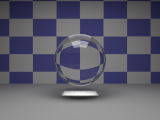
\includegraphics[width=\linewidth]{../studentTests/test13/testsuite_ref_13.png}
        \caption{PBRT-v4 renderer}
    \end{subfigure}
    \caption{Comparison of \texttt{testscene\_13} (glass refraction and Fresnel): the diffuse floor matches PBRT-v4 exactly ($0.297$), while the missing bright caustic patch beneath the sphere ($0.015$ vs $0.916$ at $(79, 93)$) and $\approx 5\%$ darker view through the glass reflect our renderer's default exclusion of caustics.}
    \label{fig:test13}
\end{figure}

\subsection{Error Handling Tests}

Error tests pass if the renderer neither crashes (signal) nor times out, and its log, \verb|stdout|, or \verb|stderr| contains a test-specific keyword—typically the offending token (e.g.\ \verb|Shpae|, \verb|cube|, \verb|velvet|, \verb|missing_texture.pfm|)—ensuring portability across other renderers. Line-number accuracy is logged but not required to pass since parsers legitimately differ. Our renderer achieved $100\%$ (17/17; Table~\ref{tab:error_tests}), reporting every defect gracefully with the exact faulty line in \verb|cgr26_expected_N.log| (representative outputs in Listing~\ref{lst:error_logs}).

\begin{table}[htbp]
\centering
\caption{Error-handling tests (\texttt{testscene\_14}--\texttt{30}): our renderer versus PBRT-v4. Our renderer passed all 17 tests and reported the exact faulty line in every case.}
\label{tab:error_tests}
\footnotesize
\renewcommand{\arraystretch}{1.12}
\setlength{\tabcolsep}{4pt}
\begin{tabularx}{\textwidth}{@{}l >{\hsize=0.95\hsize}L l >{\hsize=1.05\hsize}L@{}}
\toprule
\textbf{Scene} & \textbf{Deliberate Error} & \textbf{Ours} & \textbf{PBRT-v4 Outcome} \\
\midrule
\texttt{testscene\_14} & Unknown directive (\texttt{Shpae}) & Pass & Error, exit 1 \\
\texttt{testscene\_15} & Unknown shape (\texttt{cube}) & Pass & Error, exit 1 \\
\texttt{testscene\_16} & Malformed \texttt{Translate} & Pass & Error at line 13 (not 12), exit 1 \\
\texttt{testscene\_17} & Singular \texttt{Scale 0 1 1} & Pass & Assertion failure (\texttt{NaN} normals), exit 134 \\
\texttt{testscene\_18} & Non-numeric value (\texttt{abc}) & Pass & Error, exit 1 \\
\texttt{testscene\_19} & Missing texture (\texttt{missing\_texture.pfm}) & Pass & Error, exit 1 \\
\texttt{testscene\_20} & Missing \texttt{Include} file & Pass & Error, exit 1 \\
\texttt{testscene\_21} & Negative sphere radius & Pass & No message, renders (exit 0) \\
\texttt{testscene\_22} & Out-of-range fov ($200^\circ$) & Pass & No message, renders (exit 0) \\
\texttt{testscene\_23} & Unterminated string & Pass & Error, exit 1 \\
\texttt{testscene\_24} & Missing \texttt{]} & Pass & Error at line 13, exit 1 \\
\texttt{testscene\_25} & Wrong value count & Pass & Error, exit 1 \\
\texttt{testscene\_26} & Unmatched \texttt{AttributeEnd} & Pass & Error, ignores \& renders (exit 0) \\
\texttt{testscene\_27} & Negative resolution & Pass & Assertion failure, exit 134 \\
\texttt{testscene\_28} & Vertex index out of range & Pass & Error, then segfault (exit 139) \\
\texttt{testscene\_29} & Undefined material (\texttt{nosuchmaterial}) & Pass & Error at \texttt{Shape} line 13, exit 1 \\
\texttt{testscene\_30} & Unknown material (\texttt{velvet}) & Pass & Error, exit 1 \\
\bottomrule
\end{tabularx}
\end{table}

\begin{lstlisting}[
    float=htbp,
    caption={Representative error log outputs from \texttt{cgr26\_expected\_N.log} showing graceful detection and exact line reporting across syntax, transform, file-loading, and geometry faults.},
    label={lst:error_logs}
]
# test 14 (unknown directive)
[ERROR]   testscene_14.pbrt:12: unknown directive 'Shpae'; skipping until the next directive
...
[WARNING] render completed with 1 error(s); see messages above
[SUMMARY] 1 warning(s), 1 error(s)

# test 17 (singular scale - PBRT assertion failure)
[ERROR]   testscene_17.pbrt:13: Scale with a zero factor makes the transform singular; ignored
...
[WARNING] render completed with 1 error(s); see messages above
[SUMMARY] 1 warning(s), 1 error(s)

# test 19 (missing texture)
[ERROR]   testscene_19.pbrt:12: texture "t": cannot open image file 'missing_texture.pfm'; using magenta
...
[WARNING] render completed with 1 error(s); see messages above
[SUMMARY] 1 warning(s), 1 error(s)

# test 28 (vertex index out of range - PBRT segfault)
[ERROR]   testscene_28.pbrt:12: vertex index 7 out of range [0, 2]; shape skipped
...
[WARNING] render completed with 1 error(s); see messages above
[SUMMARY] 1 warning(s), 1 error(s)
\end{lstlisting}

\subsection{Difficulties encountered}
One major difficulty was that \verb|testscene_9| initially rendered completely black, with tests 12 and 13 sharing the same defect. Inspecting the area light quad's normal, $\mathrm{cross}(p_{10} - p_{00}, p_{01} - p_{00})$, showed that it pointed upward into the ceiling; because PBRT-v4 uses the same one-sided emission convention, the scene itself was wrong rather than the renderer. Notably, the Cornell box in \verb|testscene_12| still looked plausible beforehand due to light bouncing off the ceiling and was only caught visually. Reordering the quad vertices fixed all three scenes.

Another difficulty was that several $5 \times 5$ shading windows initially straddled shadow or checkerboard edges, making them overly sensitive to small shifts. An automated search for the smoothest nearby window fixed most of them, but drifted the penumbra pixel into the umbra and pushed both checkerboard pixels onto dark squares, so those remaining coordinates were chosen by hand from printed pixel grids.

One final difficulty was overly permissive pass criteria that could hide real regressions. During fault injection, a $9.1\%$ lighting error in \verb|testscene_8| passed under our original $0.01$ absolute tolerance, so we tightened the limit to $0.005$ for tests 8 to 11. Similarly, early error-test keywords such as \verb|]| (matching every \verb|[ERROR]| tag) and \verb|7| (matching arbitrary numbers) made those tests impossible to fail, so we restricted all keywords to specific offending tokens from each scene.

\subsection{Observations}

PBRT-v4's spectral round-trip noticeably shifts saturated emitters: pure red rendered $\approx 38\%$ brighter and blue $\approx 60\%$ dimmer (with negative channels) than our exact RGB output, whereas white lights on saturated surfaces agreed within $1.6\%$ (tests 8--11). Under multi-bounce lighting in \verb|testscene_12|, faint wall channels also diverged systematically by $10$--$18\%$ (versus $<1\%$ against our own high-sample render and $\le 0.7\%$ for direct light in \verb|testscene_10|), likely as repeated bounces amplify spectral versus RGB differences. As a result, \verb|testscene_12| passes only due to the $0.015$ absolute floor and would fail three channels under a purely relative $10\%$ rule.

In \verb|testscene_13|, disabling caustics (\verb|"bool caustics" false|) was directly measurable: at floor pixel $(79,93)$ beneath the glass sphere, PBRT peaked at $0.916$ compared to our $0.015$ ($\approx 60\times$ darker), while the non-caustic floor matched exactly ($0.297$ vs $0.297$) and the view through the sphere was $\approx 5\%$ darker.

Finally, PBRT-v4 handled our error suite inconsistently (Table~\ref{tab:error_tests}): it silently rendered invalid parameters (tests 21--22), ignored an unmatched \verb|AttributeEnd| (test 26), hit internal assertions on singular scale and negative resolution (tests 17 and 27), and segfaulted on an out-of-range vertex index (test 28), while shifting reported line numbers to the next statement or usage site on tests 16, 24, and 29.

\clearpage
\appendix

\section{BVH Parameter Tuning Results}

{\scriptsize
\setlength{\tabcolsep}{2.4pt}
\renewcommand{\arraystretch}{1.05}
\begin{longtable}{@{}llrrrrrrrrr@{}}
\caption{BVH parameter sweep ($C_t$ and maximum leaf size) across all three acceleration scenes.}
\label{tab:param_tuning_test} \\
\toprule
\textbf{Scene} & \textbf{Res.} &
\shortstack[r]{\textbf{Max}\\\textbf{leaf}} &
$\mathbf{C_t}$ &
\textbf{Nodes} &
\textbf{Leaves} &
\textbf{Depth} &
\shortstack[r]{\textbf{Build}\\\textbf{(s)}} &
\shortstack[r]{\textbf{Tests/}\\\textbf{ray}} &
\shortstack[r]{\textbf{Nodes/}\\\textbf{ray}} &
\shortstack[r]{\textbf{Render}\\\textbf{(s)}} \\
\midrule
\endfirsthead
\multicolumn{11}{@{}l}{\footnotesize\emph{Table~\thetable\ (continued)}} \\
\toprule
\textbf{Scene} & \textbf{Res.} &
\shortstack[r]{\textbf{Max}\\\textbf{leaf}} &
$\mathbf{C_t}$ &
\textbf{Nodes} &
\textbf{Leaves} &
\textbf{Depth} &
\shortstack[r]{\textbf{Build}\\\textbf{(s)}} &
\shortstack[r]{\textbf{Tests/}\\\textbf{ray}} &
\shortstack[r]{\textbf{Nodes/}\\\textbf{ray}} &
\shortstack[r]{\textbf{Render}\\\textbf{(s)}} \\
\midrule
\endhead
\midrule
\multicolumn{11}{r@{}}{\footnotesize\emph{Continued on next page}} \\
\endfoot
\bottomrule
\endlastfoot
\texttt{acc\_best}    & $1280\times 960$ & 4  & 0.125 & 4{,}095   & 2{,}048   & 12 & 0.0038 & 2.92    & 18.88   & 0.3888  \\
\texttt{acc\_best}    & $1280\times 960$ & 4  & 0.250 & 4{,}095   & 2{,}048   & 12 & 0.0037 & 2.92    & 18.88   & 0.3723  \\
\texttt{acc\_best}    & $1280\times 960$ & 4  & 0.375 & 4{,}095   & 2{,}048   & 12 & 0.0038 & 2.92    & 18.88   & 0.3705  \\
\texttt{acc\_best}    & $1280\times 960$ & 4  & 0.500 & 4{,}095   & 2{,}048   & 12 & 0.0038 & 2.92    & 18.88   & 0.3791  \\
\texttt{acc\_best}    & $1280\times 960$ & 4  & 0.625 & 4{,}095   & 2{,}048   & 12 & 0.0037 & 2.92    & 18.88   & 0.3743  \\
\texttt{acc\_best}    & $1280\times 960$ & 4  & 0.750 & 4{,}095   & 2{,}048   & 12 & 0.0036 & 2.92    & 18.88   & 0.3756  \\
\texttt{acc\_best}    & $1280\times 960$ & 4  & 0.875 & 4{,}095   & 2{,}048   & 12 & 0.0038 & 2.92    & 18.88   & 0.3728  \\
\texttt{acc\_best}    & $1280\times 960$ & 4  & 1.000 & 4{,}095   & 2{,}048   & 12 & 0.0037 & 2.92    & 18.88   & 0.3732  \\
\texttt{acc\_best}    & $1280\times 960$ & 16 & 0.125 & 4{,}095   & 2{,}048   & 12 & 0.0038 & 2.92    & 18.88   & 0.3769  \\
\texttt{acc\_best}    & $1280\times 960$ & 16 & 0.250 & 4{,}095   & 2{,}048   & 12 & 0.0037 & 2.92    & 18.88   & 0.3752  \\
\texttt{acc\_best}    & $1280\times 960$ & 16 & 0.375 & 4{,}095   & 2{,}048   & 12 & 0.0038 & 2.92    & 18.88   & 0.3740  \\
\texttt{acc\_best}    & $1280\times 960$ & 16 & 0.500 & 4{,}095   & 2{,}048   & 12 & 0.0037 & 2.92    & 18.88   & 0.3742  \\
\texttt{acc\_best}    & $1280\times 960$ & 16 & 0.625 & 4{,}095   & 2{,}048   & 12 & 0.0038 & 2.92    & 18.88   & 0.3737  \\
\texttt{acc\_best}    & $1280\times 960$ & 16 & 0.750 & 4{,}095   & 2{,}048   & 12 & 0.0037 & 2.92    & 18.88   & 0.3747  \\
\texttt{acc\_best}    & $1280\times 960$ & 16 & 0.875 & 4{,}095   & 2{,}048   & 12 & 0.0045 & 2.92    & 18.88   & 0.3736  \\
\texttt{acc\_best}    & $1280\times 960$ & 16 & 1.000 & 4{,}095   & 2{,}048   & 12 & 0.0037 & 2.92    & 18.88   & 0.3728  \\
\addlinespace
\texttt{acc\_worst}   & $640\times 480$  & 4  & 0.125 & 3{,}807   & 1{,}904   & 22 & 0.0028 & 887.69  & 2482.06 & 13.0197 \\
\texttt{acc\_worst}   & $640\times 480$  & 4  & 0.250 & 3{,}799   & 1{,}900   & 22 & 0.0025 & 888.12  & 2479.57 & 16.0991 \\
\texttt{acc\_worst}   & $640\times 480$  & 4  & 0.375 & 3{,}775   & 1{,}888   & 22 & 0.0093 & 889.82  & 2470.89 & 15.7977 \\
\texttt{acc\_worst}   & $640\times 480$  & 4  & 0.500 & 3{,}671   & 1{,}836   & 22 & 0.0026 & 902.84  & 2430.52 & 15.7648 \\
\texttt{acc\_worst}   & $640\times 480$  & 4  & 0.625 & 3{,}531   & 1{,}766   & 22 & 0.0027 & 927.46  & 2366.29 & 15.4013 \\
\texttt{acc\_worst}   & $640\times 480$  & 4  & 0.750 & 3{,}345   & 1{,}673   & 22 & 0.0026 & 967.03  & 2280.78 & 14.8637 \\
\texttt{acc\_worst}   & $640\times 480$  & 4  & 0.875 & 3{,}139   & 1{,}570   & 22 & 0.0025 & 1019.50 & 2181.46 & 13.5312 \\
\texttt{acc\_worst}   & $640\times 480$  & 4  & 1.000 & 2{,}929   & 1{,}465   & 22 & 0.0029 & 1076.72 & 2080.06 & 13.5063 \\
\texttt{acc\_worst}   & $640\times 480$  & 16 & 0.125 & 3{,}807   & 1{,}904   & 22 & 0.0032 & 887.69  & 2482.06 & 14.2043 \\
\texttt{acc\_worst}   & $640\times 480$  & 16 & 0.250 & 3{,}799   & 1{,}900   & 22 & 0.0026 & 888.12  & 2479.57 & 14.8265 \\
\texttt{acc\_worst}   & $640\times 480$  & 16 & 0.375 & 3{,}775   & 1{,}888   & 22 & 0.0026 & 889.82  & 2470.89 & 13.1570 \\
\texttt{acc\_worst}   & $640\times 480$  & 16 & 0.500 & 3{,}671   & 1{,}836   & 22 & 0.0026 & 902.84  & 2430.52 & 13.3128 \\
\texttt{acc\_worst}   & $640\times 480$  & 16 & 0.625 & 3{,}475   & 1{,}738   & 22 & 0.0025 & 944.02  & 2335.85 & 13.6173 \\
\texttt{acc\_worst}   & $640\times 480$  & 16 & 0.750 & 3{,}193   & 1{,}597   & 19 & 0.0024 & 1018.99 & 2195.49 & 13.2584 \\
\texttt{acc\_worst}   & $640\times 480$  & 16 & 0.875 & 2{,}801   & 1{,}401   & 19 & 0.0025 & 1137.31 & 1991.95 & 14.8312 \\
\texttt{acc\_worst}   & $640\times 480$  & 16 & 1.000 & 2{,}499   & 1{,}250   & 19 & 0.0024 & 1241.24 & 1825.49 & 14.9423 \\
\addlinespace
\texttt{acc\_complex} & $640\times 480$  & 4  & 0.125 & 314{,}183 & 157{,}092 & 24 & 0.3271 & 2.66    & 19.25   & 3.9601  \\
\texttt{acc\_complex} & $640\times 480$  & 4  & 0.250 & 314{,}183 & 157{,}092 & 24 & 0.3144 & 2.66    & 19.25   & 3.9716  \\
\texttt{acc\_complex} & $640\times 480$  & 4  & 0.375 & 314{,}025 & 157{,}013 & 24 & 0.3085 & 2.66    & 19.25   & 3.9616  \\
\texttt{acc\_complex} & $640\times 480$  & 4  & 0.500 & 314{,}015 & 157{,}008 & 24 & 0.3106 & 2.66    & 19.25   & 3.9547  \\
\texttt{acc\_complex} & $640\times 480$  & 4  & 0.625 & 313{,}903 & 156{,}952 & 24 & 0.3313 & 2.66    & 19.25   & 3.9905  \\
\texttt{acc\_complex} & $640\times 480$  & 4  & 0.750 & 313{,}231 & 156{,}616 & 24 & 0.3051 & 2.66    & 19.24   & 3.9637  \\
\texttt{acc\_complex} & $640\times 480$  & 4  & 0.875 & 312{,}079 & 156{,}040 & 24 & 0.3101 & 2.66    & 19.24   & 3.9965  \\
\texttt{acc\_complex} & $640\times 480$  & 4  & 1.000 & 307{,}231 & 153{,}616 & 24 & 0.3194 & 2.67    & 19.22   & 3.9441  \\
\texttt{acc\_complex} & $640\times 480$  & 16 & 0.125 & 314{,}183 & 157{,}092 & 24 & 0.3212 & 2.66    & 19.25   & 3.9318  \\
\texttt{acc\_complex} & $640\times 480$  & 16 & 0.250 & 314{,}183 & 157{,}092 & 24 & 0.3465 & 2.66    & 19.25   & 4.0285  \\
\texttt{acc\_complex} & $640\times 480$  & 16 & 0.375 & 314{,}025 & 157{,}013 & 24 & 0.3118 & 2.66    & 19.25   & 3.9816  \\
\texttt{acc\_complex} & $640\times 480$  & 16 & 0.500 & 314{,}015 & 157{,}008 & 24 & 0.3246 & 2.66    & 19.25   & 3.8339  \\
\texttt{acc\_complex} & $640\times 480$  & 16 & 0.625 & 313{,}903 & 156{,}952 & 24 & 0.3192 & 2.66    & 19.25   & 3.9136  \\
\texttt{acc\_complex} & $640\times 480$  & 16 & 0.750 & 313{,}231 & 156{,}616 & 24 & 0.3056 & 2.66    & 19.24   & 3.9695  \\
\texttt{acc\_complex} & $640\times 480$  & 16 & 0.875 & 312{,}035 & 156{,}018 & 24 & 0.3117 & 2.66    & 19.24   & 3.9120  \\
\texttt{acc\_complex} & $640\times 480$  & 16 & 1.000 & 307{,}107 & 153{,}554 & 24 & 0.3235 & 2.67    & 19.22   & 3.9941  \\
\end{longtable}
}

\end{document}